\documentclass[12pt]{ctexart}
\usepackage[doublespacing]{setspace}
\usepackage{amsmath, amssymb}
\usepackage{graphicx}

\begin{document}

\begin{center}
    \large \textbf{智能手机销量随价格变化关系探究}

    林绍钦 518021910331
\end{center}                               

\section{摘要}

    智能手机市场经过了几十年来的进化,从直板机、翻盖机到如今的全面屏手机、折叠屏手机。随着普及度越来越高,价格范围也越来越广。虽说消费者在购买手机时会受到多种因素的影响,但若是将考虑范围限定在同一品牌的手机中,便可以忽视品牌、消费人群等因素,单纯考虑\textbf{销量与手机价位的关系}。

    本文选取了\textbf{近三年来苹果手机iPhone在京东平台的销售数据},以某台售出手机的价格为随机变量,构造随机变量序列。在中心极限定理的保证下,该随机变量序列应服从正态分布;通过估计正态分布参数,得出均值和方差;通过理论计算所得的均值和方差,对苹果产品定价的合理性进行评估,并分析其它因素存在的影响。

    \newpage
\section{正文}

    \subsection{数据收集}

        \subsubsection{青睐价位数据}   

            根据京东手机页面销售数据:将手机价格划分为廉价(1-349)、低(349-1362)、中(1362-3573)、高(3573-8096)、昂贵(大于8096)(单位/元),对应手机消费者青睐比例如下表所示:

            \begin{center}
                \begin{tabular}{|c|ccccc|}
                    \hline
                    价格划分&廉价&低&中&高&昂贵\\
                    \hline
                    青睐比例&0.08&0.29&0.43&0.15&0.05\\
                    \hline
                \end{tabular}
            \end{center}
        \subsubsection{各季度iPhone销量}
            根据macstories网站整理,iPhone四季度销量呈周期性变化,且规律较为统一。
            \begin{center}
                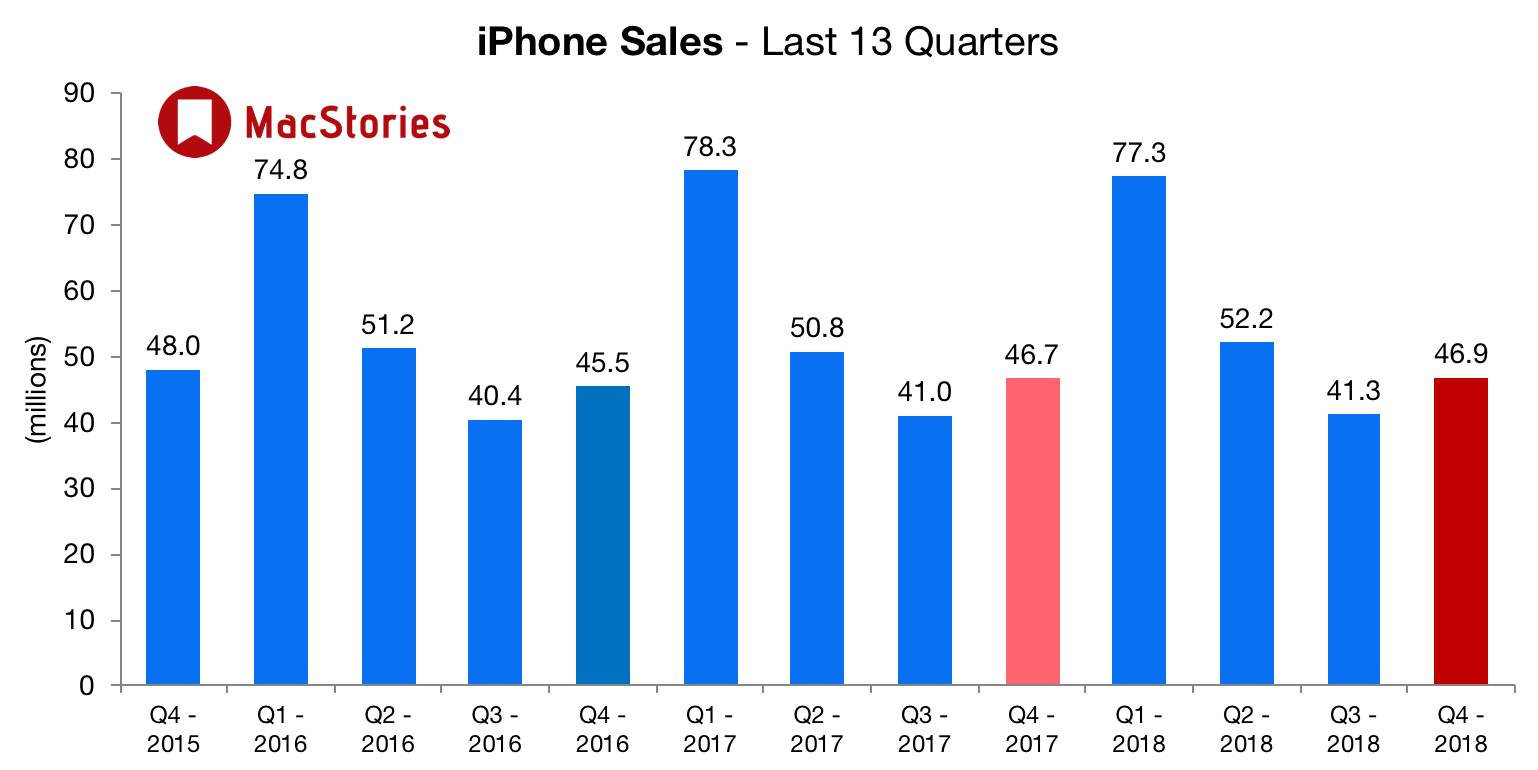
\includegraphics[width=13cm]{quarters.jpg}
            \end{center}
            
        \subsubsection{各产品总销量}
            每款iPhone销量通过京东的评价数得出;
            其价格通过软件「慢慢买」得出售价的波动曲线。
                
            2019.9上市机型:
            \begin{center}
                \begin{tabular}{|c|cc|}
                    \hline
                     & 上市价格/元 & 总销量/万台 \\
                    \hline
                    iPhone 11 &5999 &70 \\
                    \hline
                    iPhone 11 Pro&9999 &13\\
                    \hline
                    iPhone 11 ProMax&10899 &12\\
                    \hline
                \end{tabular}
            \end{center}

                2018.9上市机型:
            \begin{center}
                \begin{tabular}{|c|cc|}
                    \hline
                     & 上市价格/元 & 总销量/万台 \\
                    \hline
                    iPhone XR  &6999 &208 \\
                    \hline
                    iPhone Xs &8699 &36\\
                    \hline
                    iPhone Xs Max&10999 &103\\
                    \hline
                \end{tabular}
            \end{center}

                2017.9上市机型:
            \begin{center}
                \begin{tabular}{|c|cc|}
                    \hline
                     & 上市价格/元 & 总销量/万台 \\
                    \hline
                    iPhone 8 &4777 &152 \\
                    \hline
                    iPhone 8 Plus &6899 &199\\
                    \hline
                \end{tabular}
            \end{center}

\newpage

\subsection{数据处理与参数估计}

    \subsubsection{价位青睐分布}

        将消费者对价位段的选择看作离散型随机变量,取区间最小值为代表,
        并且由Khintchine大数定律的保证,在n较大时(京东月销量80w台手机),可以用频率作为对未知参数的估计,得到随机变量的分布列。

        \begin{center}
            \begin{tabular}{|c|ccccc|}
                \hline
                $X _i$&1&349&1362&3573&8096\\
                \hline
                $p _i$&0.08&0.29&0.43&0.15&0.05\\
                \hline
            \end{tabular}
        \end{center}    

        \textbf{期望计算} :
        \begin{equation} %推荐使用equation表达式  
            E (X)= \sum_{i = 1}^{5} X _i \cdot p _i = 1642.70
        \end{equation} 
        
        该结果表明,1642.70元附近是消费者最为青睐的价位。
        经过分析,由于价格变化可近似为指数变化,故取价格的自然对数后再取期望:
        \begin{equation} %推荐使用equation表达式  
            e^{E (lnX)} = 653.53
        \end{equation} 
        即在考虑价格分布的不均匀程度后,对于整体手机销售情况而言,653.53元附近是消费者最为青睐的价位。

        \textbf{方差、标准差计算}:
        \begin{equation} %推荐使用equation表达式  
            D (X)=   EX^2 - E^2X= 3435428.15
        \end{equation} 
        \begin{equation} %推荐使用equation表达式  
            \sigma _X =   \sqrt{D (X)}  = 1853.49
        \end{equation}
       
\newpage

    \subsubsection{价格与折算销量关系分析}
        因iPhone四季度销量呈周期性变化,且规律较为统一。所以可对不同批次发布的产品的销量加权后进行比较,权值通过取三年每季度总销量和三年总销量之比获得。
        \begin{equation} %推荐使用equation表达式  
            \alpha _i= \frac{\sum\limits_{k = 2016}^{2018} E _{ki} }{ \sum\limits_{k = 2016}^{2018} \sum\limits_{j = 1}^{4}E _{kj} }, \qquad i=1,2,3,4
        \end{equation} 
        其中$\alpha _i$表示第$i$个季度的权值,$E _{ki}$ 为$k$年第$i$季度的销量。
        \begin{center}
            \begin{tabular}{|c|c|c|c|c|}
                \hline
                季度 $i$ & 一&二&三&四\\
                \hline
                权重 $\alpha _i$&0.356 &0.239&0.190 &0.215\\
                \hline
            \end{tabular}
        \end{center}
        \begin{center}
            %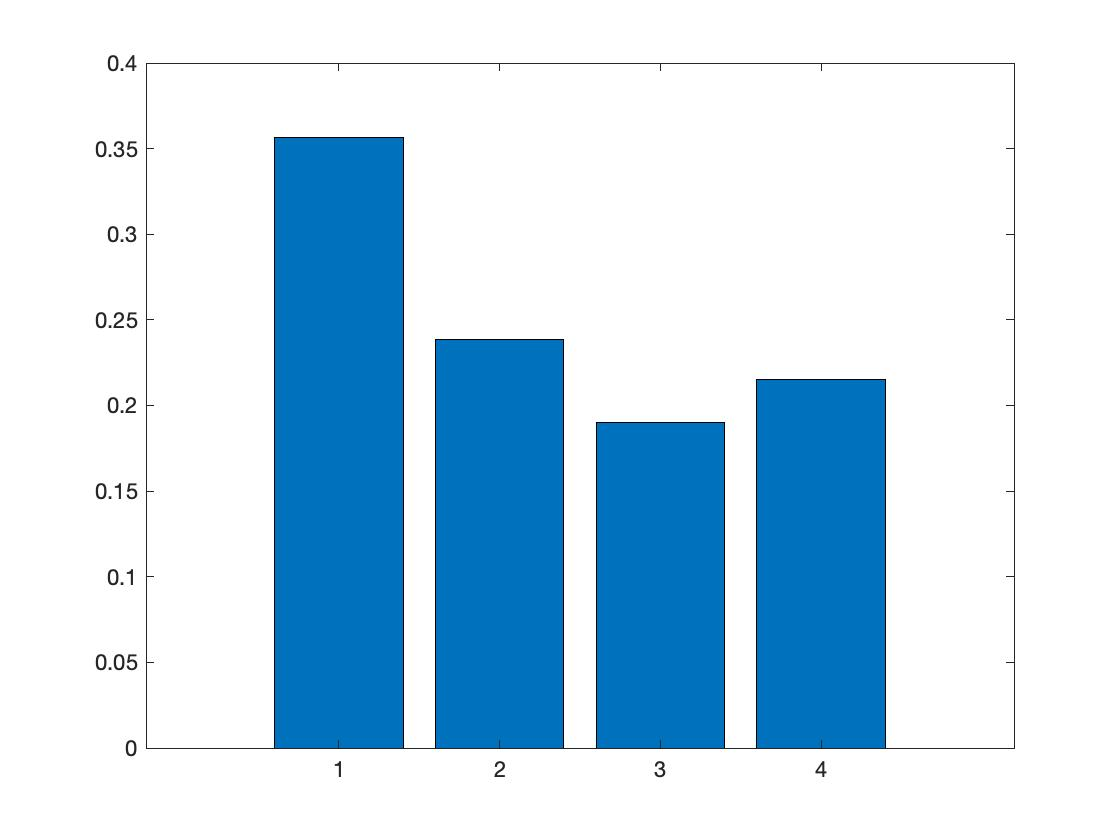
\includegraphics[width=9cm]{per-quaters.jpg}
        \end{center}    
        因新手机在上市第一季度售价相对稳定,通过四季度销量分布可以折算出每款手机在发布后第一个季度的销量(即第四季度),使不同时间发布的手机具有一定的可比性。

        \begin{equation} %推荐使用equation表达式  
            E _i ' = \alpha _4 \cdot  E _i
        \end{equation} 

            
        \begin{center}
            \begin{tabular}{|c|c|c|}
                \hline
                机型 & 上市价格/元 &折算销量$E _i$/万台\\
                \hline
                iPhone 11 &5999 &70\\
                \hline
                iPhone 11 Pro&9999 &13\\
                \hline
                iPhone 11 ProMax&10899 &12\\
                \hline
                iPhone XR  &6999  &44\\
                \hline
                iPhone Xs &8699 &7\\
                \hline
                iPhone Xs Max&10999 &22\\
                \hline
                iPhone 8 &4777&21\\
                \hline
                iPhone 8 Plus &6899&32\\
                \hline
            \end{tabular}
        \end{center}

        \textbf{矩估计法}:
        在不清楚随机变量分布的情况下,用矩估计法(原点矩)对期望和方差进行初步估计
        \begin{equation} %推荐使用equation表达式  
            \mu _1= \frac{1}{n} \sum_ {i=1}^{n} X _i = 7035.20 =\mu
        \end{equation} 
        \begin{equation} %推荐使用equation表达式  
            \mu _2= \frac{1}{n} \sum_ {i=1}^{n} X _i^2 = 5.267 \times 10^7=\sigma ^2 + \mu ^2
        \end{equation} 
        \begin{equation} %推荐使用equation表达式  
            \mu = 7035.20 
        \end{equation} 
        \begin{equation} %推荐使用equation表达式  
            \sigma ^2 = 3.183\times 10^6,\qquad \sigma = 1784.30
        \end{equation} 
        
        \newpage
        \textbf{最大似然估计法}:
        以某台售出手机的价格为随机变量,构造随机变量序列$\{X _n\}$,依照中心极限定理,当n很大时(总折算销量达到了221万台),该随机变量序列应服从正态分布。
    在中心极限定理的保证下,随机变量序列应服从正态分布。因此可以通过随机变量序列求总体$N(\mu, \sigma^2)$ 中$\mu$和$\sigma$的最大似然估计值。

        解正态总体的似然方程组,易得最大似然估计量为:
        \begin{equation}
            \hat{\mu} = \frac{1}{n} \sum_ {i=1}^{n} X _i 
        \end{equation}
        \begin{equation}
            \hat{\sigma}^2 = \frac{1}{n} \sum_ {i=1}^{n} (X _i - \bar{X})^2 
        \end{equation}

        带入样本观察值,得到最大似然估计值为:
        \begin{equation} %推荐使用equation表达式  
            \mu = 7035.20 
        \end{equation} 
        \begin{equation} %推荐使用equation表达式  
            \sigma ^2 = 3.183\times 10^6,\qquad \sigma = 1784.30
        \end{equation} 
        
        易观察得,正态总体的最大似然估计量与矩估计量形式相同,因而估计值也相同。

    
    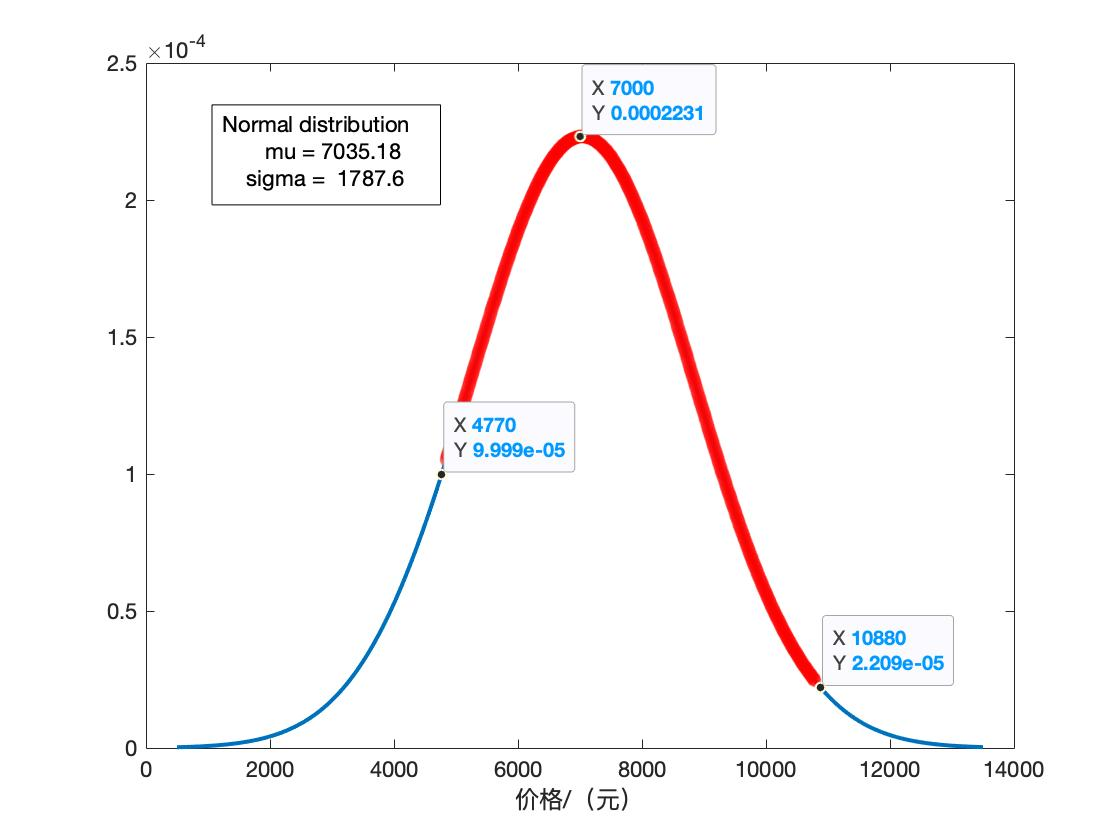
\includegraphics[width=12cm]{price_normal_distribution.jpg}

    图中标红区域为iPhone价格所覆盖的区域,最低和最高售价以及最高销量点对应售价如图所示。

    \newpage

\section{分析与结论}

    虽然影响销量的因素很多,但价格的确能决定销量的走向。将所有iPhone的出售价格作为随机变量序列,可以近似看作服从正态分布。
    
    根据正态分布曲线,低于7000元的iPhone机型可以适当涨价,以获取更高的总利润。而高于7000元的机型需要权衡利润与销量的关系,再对售价进行调整。

    根据2.2.1中对\textbf{所有手机销售情况的价格青睐程度}的分析,与2.2.2中对\textbf{iPhone手机价格与折算销量关系}的分析相比,可以明显发现iPhone售价期望要远高于一般手机,且iPhone消费者的购买力强于所有的手机消费者的平均购买力。

    

    

\newpage

\begin{thebibliography}{99}

    [1]  \textsl{《概率论与数理统计》}, 上海交通大学出版社

    \newline

    [2]  \textsl{https://www.macstories.net}  , Apple news, app reviews, and stories by Federico Viticci and friends.

    \newline

    [3] \textsl{https://shouji.jd.com} , 手机-京东商城

\end{thebibliography}

\end{document}

